 \chapter{Literature review}

\section{USAR}

\section{USAR Robots}

\section{Load-Intuitive Modules}

\begin{wrapfigure}{r}{0.35\textwidth} %this figure will be at the right
	\centering
	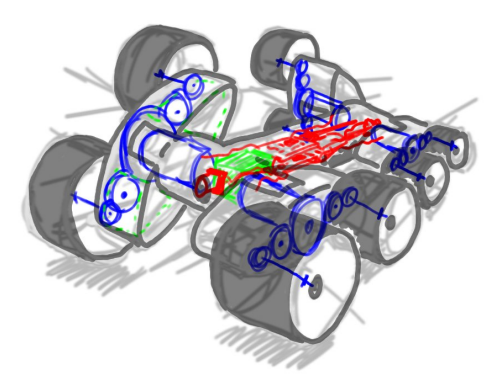
\includegraphics[width=0.35\textwidth]{Wilson-sketch}
	\caption{Systems layout of Wilson's LIM device \citep{Wilson-2013}}
	\label{Wilson sketch-lit}
\end{wrapfigure}

A Load-Intuitive Module (LIM) refers to a wheel system proposed by Matthew Wilson, shown in Figure \ref{Wilson sketch-lit} \citep{Wilson-2013}. The LIM system uses a two outer "minor wheels" placed on a central hub that can be rotated as a "major wheel". The minor wheels are geared to the central hub such that they drive the vehicle, however if they experience high resistance, for example from hitting an obstacle, the torque will cause the major wheel to rotate instead, flipping one of the minor wheels over the obstacle to automatically climb it. The system is referred to as "Load-Intuitive" because it will intuitively climb over obstacles in response to increased load on the wheels. LIMs are designed to be used in low cost USAR robots, allowing them to climb over objects without the need for many actuators.

\noindent "LIMed" robot platforms (platforms using LIMs for locomotion) were built individually by four final year students at UCT \citep{Wilson-2013},  \citep{Haskel-2017}, \citep{Buchanan-2018}, and \citep{Powrie-2019-lit}. One of these robots is shown in Figure \ref{Powrie robot}. These platforms show some success in climbing a single step, albeit inconsistently. None of the previous students were able to build a full system such that they can perform extensive tests on the system.


\begin{figure}[h]
	\centering
	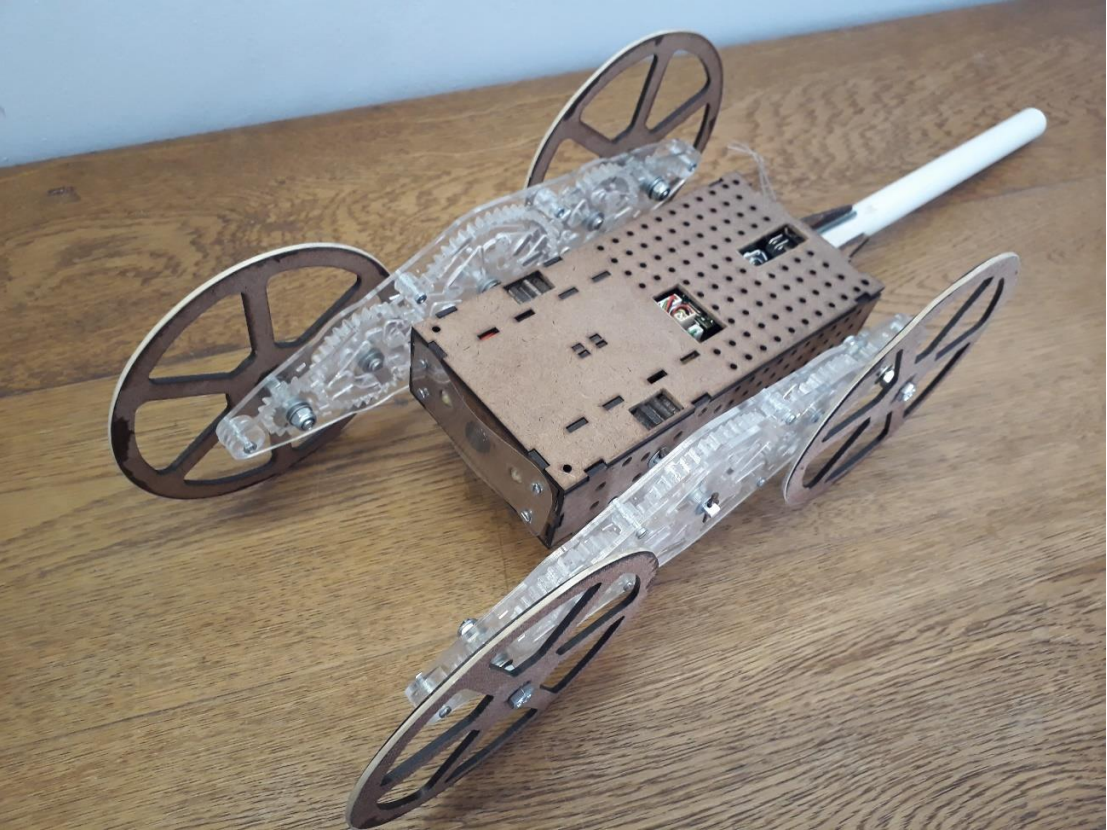
\includegraphics[width=0.8\textwidth]{Powrie-device}
	\caption{Powrie's "Di-Wheel" robot \citep{Powrie-2019}}
	\label{Powrie robot-lit}
\end{figure}
